
% ----------------------------------------------------------------------
%  Set the document class
% ----------------------------------------------------------------------
\documentclass[11pt,a4paper,twoside]{article}

% ----------------------------------------------------------------------
% Define external packages, language, margins, fonts and new commands
% ----------------------------------------------------------------------
%\input{preamble} 
\usepackage[utf8]{inputenc}   % <<<<< Linux
\usepackage[english]{babel} % <<<<< English
\usepackage{notoccite}
\usepackage[skip=0.5\baselineskip]{caption}
\hyphenation{GTKWave}
\usepackage{listings}
\usepackage[all]{nowidow}
\usepackage{amsmath}
\usepackage{systeme}

%blind text
\usepackage{lipsum}

\usepackage{graphicx}
\graphicspath{{./}{../../figlib/}{../mat/}{../sim/}}
\def\FontLn{% 16 pt normal
  \usefont{T1}{phv}{m}{n}\fontsize{16pt}{16pt}\selectfont}
\def\FontLb{% 16 pt bold
  \usefont{T1}{phv}{b}{n}\fontsize{16pt}{16pt}\selectfont}
\def\FontMn{% 14 pt normal
  \usefont{T1}{phv}{m}{n}\fontsize{14pt}{14pt}\selectfont}
\def\FontMb{% 14 pt bold
  \usefont{T1}{phv}{b}{n}\fontsize{14pt}{14pt}\selectfont}
\def\FontSn{% 12 pt normal
  \usefont{T1}{phv}{m}{n}\fontsize{12pt}{12pt}\selectfont}

% Use Arial font as default
%
\renewcommand{\rmdefault}{phv}
\renewcommand{\sfdefault}{phv}
\usepackage{geometry}	
\geometry{verbose,tmargin=2.5cm,bmargin=2.5cm,lmargin=2.5cm,rmargin=2.5cm}

%\usepackage{setspace}
%\renewcommand{\baselinestretch}{1.5}

\usepackage[pdftex]{hyperref} % enhance documents that are to be
                              % output as HTML and PDF
\hypersetup{colorlinks,       % color text of links and anchors,
                              % eliminates borders around links
%            linkcolor=red,    % color for normal internal links
            linkcolor=black,  % color for normal internal links
            anchorcolor=black,% color for anchor text
%            citecolor=green,  % color for bibliographical citations
            citecolor=black,  % color for bibliographical citations
%            filecolor=magenta,% color for URLs which open local files
            filecolor=black,  % color for URLs which open local files
%            menucolor=red,    % color for Acrobat menu items
            menucolor=black,  % color for Acrobat menu items
%            pagecolor=red,    % color for links to other pages
            pagecolor=black,  % color for links to other pages
%            urlcolor=cyan,    % color for linked URLs
            urlcolor=black,   % color for linked URLs
	          bookmarks=true,         % create PDF bookmarks
	          bookmarksopen=false,    % don't expand bookmarks
	          bookmarksnumbered=true, % number bookmarks
	          pdftitle={report},
            pdfauthor={Andre C. Marta},
%            pdfsubject={Thesis Title},
%            pdfkeywords={Thesis Keywords},
            pdfstartview=FitV,
            pdfdisplaydoctitle=true}

\usepackage[numbers,sort&compress]{natbib} % <<<<< References in numbered list [1],[2],...
\usepackage{subcaption} 
\usepackage{mdframed}

%%%%%%%%%%%%%%%%%%%%%%%%%%%%%%%%%%%%%%%%%%%%%%%%%%%%%%%%%%%%%%%%%%%%%%%%
%     Begin Document                                                   %
%%%%%%%%%%%%%%%%%%%%%%%%%%%%%%%%%%%%%%%%%%%%%%%%%%%%%%%%%%%%%%%%%%%%%%%%


\begin{document}

% Set plain page style (no headers, footer with centered page number)
\pagestyle{plain}

% Set roman numbering (i,ii,...) before the start of chapters
%\pagenumbering{roman}

% ----------------------------------------------------------------------
%  Cover page
% ----------------------------------------------------------------------
%%%%%%%%%%%%%%%%%%%%%%%%%%%%%%%%%%%%%%%%%%%%%%%%%%%%%%%%%%%%%%%%%%%%%%%%
%                                                                      %
%     File: Thesis_FrontCover.tex                                      %
%     Tex Master: Thesis.tex                                           %
%                                                                      %
%     Author: Andre C. Marta                                           %
%     Last modified :  2 Jul 2015                                      %
%                                                                      %
%%%%%%%%%%%%%%%%%%%%%%%%%%%%%%%%%%%%%%%%%%%%%%%%%%%%%%%%%%%%%%%%%%%%%%%%

\thispagestyle {empty}

% IST Logo - Signature A
% parameters: bb=llx lly urx ury (bounding box), width=h_length, height=v_length, angle=angle, scale=factor, clip=true/false, draft=true/false. 
\includegraphics[bb=9.5cm 11cm 0cm 0cm,scale=0.29]{IST_A_CMYK_POS}

\begin{center}
%
% Figure (Image or plot)
\vspace{1.0cm}
% height = 50 mm
%\includegraphics[height=50mm]{Figures/Airbus_A350.jpg}

% Title, author and degree
\vspace{1cm}
{\FontLb Circuit Theory and Electronics Fundamentals} \\ % <<<<< EDIT TITLE
\vspace{1cm}
{\FontSn Mestrado em Engenharia Física Tecnológica, Técnico, University of Lisbon} \\ % <<<<< EDIT COURSE
\vspace{1cm}
{\FontSn Ana Martins (96506), Miguel Moreira (96556), Sara Oliveira (96566)} \\
\vspace{1cm}
{\FontSn T5} \\
\vspace{1cm}
{\FontSn May 5, 2021} \\ % <<<<< EDIT DATE (corresponds to date of oral examination)
%
\end{center}



% ----------------------------------------------------------------------
% Dedication page (optional)
% ----------------------------------------------------------------------
%\input{dedication} 
%\cleardoublepage

% ----------------------------------------------------------------------
%  Acknowledgments (optional)
% ----------------------------------------------------------------------
%\input{acknowledgements}
%\cleardoublepage

% ----------------------------------------------------------------------
%  Abstract (both in English and Portuguese)
% ----------------------------------------------------------------------
%\input{resumo} 
%\cleardoublepage

%\input{abstract} 

% ----------------------------------------------------------------------
%  Table of contents, list of tables, list of figures and nomenclature
% ----------------------------------------------------------------------

% Table of contents
%
\tableofcontents

% List of tables
%\addcontentsline{toc}{section}{\listtablename}
%\listoftables
%\cleardoublepage 

% List of figures
%\addcontentsline{toc}{section}{\listfigurename}
%\listoffigures
%\cleardoublepage 

% Set arabic numbering (1,2,...) after preface
%
%\setcounter{page}{1}
%\pagenumbering{arabic}

% ----------------------------------------------------------------------
%  Body
% ----------------------------------------------------------------------

\newpage
\section{Introduction}
\label{sec:introduction}

% state the learning objective 
The objective of this laboratory assignment is to study a circuit containing an Independent AC Voltage Souce, $V_s(t)$, a Voltage Controlled Current Source, $I_d$, a Current Controlled Voltage Source, $V_d$, a Capacitor $C$, and seven resistors, $R_1$ to $R_7$. The circuit that we were first presented with is displayed in Figure \ref{fig:circ}, with some added current directions to ease the process of finding equations in our Analysis section. As we make modifications to the circuit along the report to suit our needs, the circuit used for those will also be displayed.

\begin{figure}[h] \centering
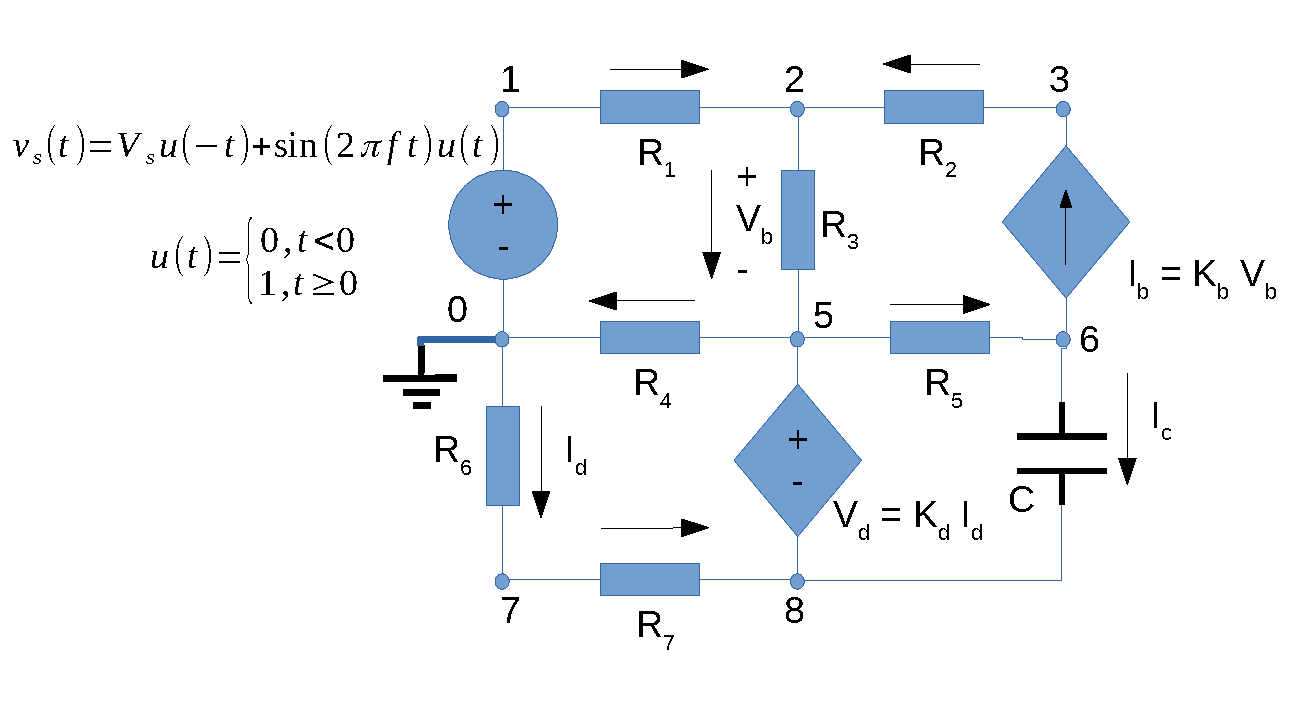
\includegraphics[width=0.6\linewidth]{t2-original.pdf}
\caption{The original circuit, with some current directions added.}
\label{fig1}
\end{figure}

In Section~\ref{sec:analysis}, a theoretical analysis of the circuit is
presented, including the study of what happens for $t<0$, finding the the equivalent resistor as seen from the capacitor
terminals, the natural and forced solutions of the circuit in $t>0$, as well as frequency analysis.

In Section~\ref{sec:simulation}, the circuit is analysed by
simulation using the \textit{software Ngspice}, ultimately, studying the same as in the Theoretical Analysis section.
The results in each Analsysis are compared \ref{sec:comparing}.
The conclusions of this study are outlined in
Section~\ref{sec:conclusion}.


\section{Theoretical Analysis}
\label{sec:analysis}

In this section, the circuit shown in Figure~\ref{fig1} is analysed via node analysis and mesh analysis.

\subsection{Node analysis}



Labels were assigned to identify nodes from zero to seven, to then proceed with the mesh and node analysis (the 0th of which being the ground). This is helpful because we can, therefore, derive direct equations in terms of the voltage at these nodes.

The voltage $V_i$ refers to the node $i$. For this procedure, one applies KCL (Kirchoff's Current Law), which states that the sum of currents leaving a node must be the same as the sum of currents entering a node. It's relevant to notice that this kind of approach is only possible for the nodes which aren't directly connected to a terminal of a voltage source, therefore, we can only derive 4 of these equations: in that case, it's crucial to find other equations to cover all the unknown variables of the system. The approach is then to consider the voltage gain between to nodes that have a voltage source between them: for example, the nodes 5 and 0 are connected to $V_c$, which means $V_5 = V_c + V_0$, which wields us the $7^{th}$ equation in~\ref{eq:1}. Moreover, we can relate the currents associated with the controlled sources with the nodes we numerated: for example, in $I_c$ there is a voltage drop, which gives us the $6^{th}$ equation.
The current flow direction is considered, whenever possible, the same as indicated by each $I_i$, with $i$ ranging from 1 to 4, as shown in~\ref{fig1}. The cases where this is not possible are the currents going through nodes 2 to 5 and 5 to 6; for these, we considered, respectively, the direction of $V_b$ and of $I_d$.

The equations are as follows

\begin{equation} 
\begin{cases}  
    Node\, 2: \frac{V_1 - V_2}{R_1} + \frac{V_2 - V_5}{R_3} + \frac{V_2 - V_3}{R_2} = 0 \\
    Node\, 3: \frac{V_2 - V_3}{R_2} + I_b = 0 \\
    Node\, 6: \frac{V_6 - V_5}{R_5} - I_b = \,  - I_d \\
    Node\, 7: \frac{V_7 - V_4}{R_6} - \frac{V_7}{R_7} = 0 \\
    \frac{V_2 - V_5}{R_3} - I_b = 0 \\
    \frac{V_4 - V_7}{R_6} - I_c = 0\\
    V_5 - V_c = 0\\
\end{cases}
\label{eq:1}
\end{equation}

\subsection{Mesh analysis}


In the mesh analysis, every mesh is given an arbitrary current ($I_1$, $I_2$, $I_3$, $I_4$), represented in Figure~\ref{fig1} with round arrows. This is helpful because we can, therefore, derive direct equations in terms of the current passing through these meshes.

The current $I_i$ refers to the mesh $i$. For this method, we apply KVL (Kirchoff's Voltage Law), which states that the sum of all the voltages around any closed loop in a circuit is equal to zero, and relate the fictional currents we created to currents given in the circuit (for example, $I_d$).

This can't be done for every mesh as the Law would specifically entail, but we can reach conclusions about every one of them by inspection of said mesh: for example, the $2^{nd}$ mesh is connected to a current source, which automatically wields the $2^{nd}$ equation.

The equations are as follows

\begin{equation} 
\begin{cases}  
    Mesh\, 1: R_1\,I_1 + R_3\,(I_1 - I_2) + R_4(I_1 - I_3) = V_a \\
    Mesh\, 2: I_2 + I_b = 0\\
    Mesh\, 3: R_4(I_3 - I_1) + V_c + R_7\,I_3 + R_6\,I_3 = 0 \\
    Mesh\, 4: I_4 = -I_d \\
    R_3\, (I_1 - I_2) - V_b = 0\\
    I_3 + I_c = 0 \\

\end{cases}
\label{eq:2}
\end{equation}

\subsection{Circuit Solution}

To make sense out of the equations that were presented already, we also have to add

\begin{equation} 
\begin{cases}  
   K_b\,V_b - I_b = 0 \\
  K_c\, I_c - V_c = 0 \\
\end{cases}
\label{eq:3}
\end{equation}

We then use \textit{GNU Octave}, a $software$ that can solve this system of equations, to obtain the values of all the unknowns. Knowing all the voltages allows us to know every current as well, which means the circuit is solved.
The results of these computations are compiled in this table.

\begin{table}[h]
  \centering
  \begin{tabular}{|l|r|}
    \hline    
    {\bf Name} & {\bf Value [A and V]} \\ \hline
    V1 & 7.1581440e+00\\\hline V2 & 7.1581440e+00\\\hline V3 & 6.6424218e+00\\\hline V4 & 9.9835499e-01\\\hline V5 & 7.9316995e+00\\\hline V6 & 4.0555787e+00\\\hline V7 & -9.7816698e-01\\\hline Vb & -3.5456366e-02\\\hline Vc & 7.9316995e+00\\\hline I1 & 2.3690260e-04\\\hline I2 & 2.4828279e-04\\\hline I3 & -9.7373690e-04\\\hline I4 & -1.0314759e-03\\\hline Ib & -2.4828279e-04\\\hline Ic & 9.7373690e-04\\\hline 
  \end{tabular}
  \caption{Node and Mesh Analysis Computation Results. A variable starting with I is of type {\em current}
    and expressed in Ampere; a variable starting with V is of type {\it voltage} and expressed in
    Volt.}
  \label{tab:op}
\end{table}

\section{Simulation Analysis}
\label{sec:simulation}

\subsection{Operating Point Analysis}

Table~\ref{tab:op} shows the simulated operating point results for the circuit under analysis.

\begin{table}[htb!]
  \centering
  \begin{tabular}{|l|r|}
    \hline    
    {\bf Name} & {\bf Value [A or V]} \\ \hline
    @gb[i] & -2.48284e-04\\ \hline
@r1[i] & 2.369027e-04\\ \hline
@r2[i] & -2.48284e-04\\ \hline
@r3[i] & -1.13810e-05\\ \hline
@r4[i] & 1.210640e-03\\ \hline
@r5[i] & -2.48284e-04\\ \hline
@r6[i] & 9.737374e-04\\ \hline
@r7[i] & 9.737374e-04\\ \hline
v(1) & 5.185042e+00\\ \hline
v(2) & 4.941554e+00\\ \hline
v(3) & 4.425830e+00\\ \hline
v(5) & 4.977013e+00\\ \hline
v(6) & 5.729012e+00\\ \hline
v(7) & -1.97652e+00\\ \hline
v(8) & -2.95469e+00\\ \hline
v(9) & 0.000000e+00\\ \hline

  \end{tabular}
  \caption{Operating point results. A variable preceded by @ is of type {\em current}
    and expressed in Ampere; other variables are of type {\it voltage} and expressed in
    Volt.}
  \label{tab:op}
\end{table}

These results were produced using the \textit{Ngspice software}. In order for the \textit{software} to be able to recognise the Current-Controlled Voltage Source, defined in Figure \ref{fig2} as $H_c$, we had to add a new Independent Voltage Source with a voltage of 0V, which is also represented in \ref{fig2}.


\begin{figure}[h] \centering
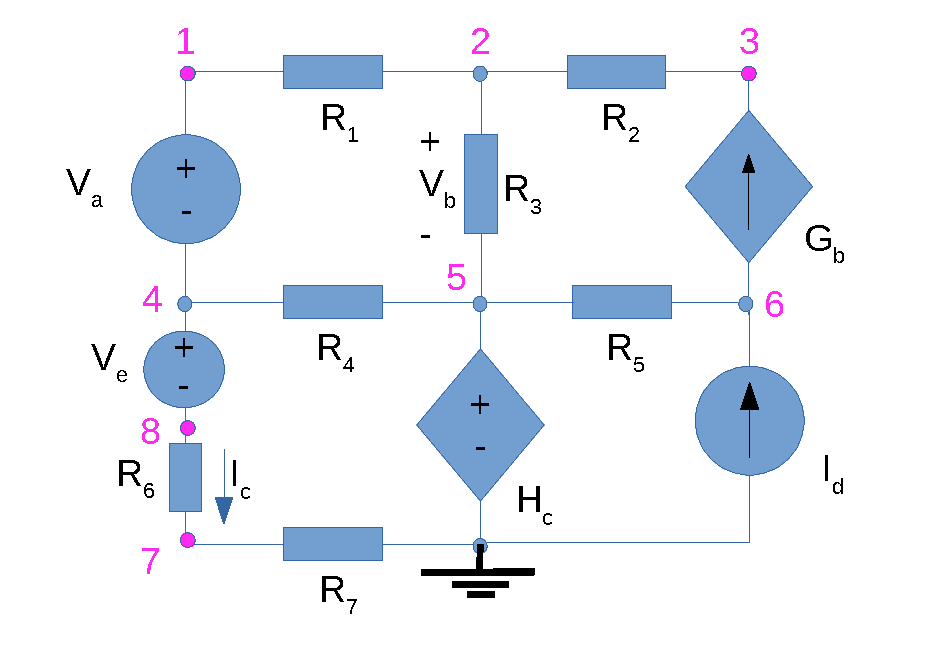
\includegraphics[width=0.4\linewidth]{t1-2.pdf}
\caption{The original circuit with an added voltage source of value 0V.}
\label{fig2}
\end{figure}


To compare the results between the theoretical calculations and the simulation it's important to keep in mind that the current values and directions represented in \ref{fig2} by round arrows: $I_1$ $I_2$ $I_3$ e $I_4$ correspond, respectively, to the following values in the simulation data table (\ref{tab:op}): @r1[i], -@r2[i], -@id[current], -@r6[i] (or @r7[i], they're equivalent).


On a general basis, the values obtained by the simulation greatly resemble the ones obtained using the theoretical models and the application \textit{GNUOctave} to compute them.

In fact, by inspection it's possible to conclude that pratically all the values fit in the same magnitude as its correspondent. The biggest absolute difference reports to the voltage in node six, v(6): theoretical value - 4.0555787e+00 V, simulated value: 1.180782e+01 V. Being the biggest divergence, this represents an absolute error (|theoretical - simulated|/) of 7.752241 V.

\clearpage
\section{Conclusion}
\label{sec:conclusion}



In this laboratory assignment the objective of analysing a circuit with several current and voltage sources (two linearly
dependent and one independent) and a capacitor in parallel and in series with resistors has been
achieved.

The current and voltage theoretical analysis (computed using \textit{GNUOctave}) precisely resembles the
circuit simulated by the \textit{Ngspice}. 

As seen in the previous section, it's possible to conclude that the simulations follows very closely the theorical model
used in the analysis: the node analysis.

To conclude, we find that the study of the circuit we were present with was successful.

\begin{thebibliography}{}

\bibitem{slides-ngspice}
Phyllis R. Nelson, \emph{Introduction to SPICE Source Files} Slides

\bibitem{spice-stanford}
\emph{SPICE 'Quick' Reference Sheet}, Stanford University

\bibitem{ngspice-guide}
Holger Vogt \textit{et al}, \emph{Ngspice's User Manual}, Version 34

\bibitem{octave}
\emph{GNU Octave} Documentation Files 

\bibitem{slides-prof}
José Teixeira de Sousa, \emph{Circuit Theory and and Eletronic Fundamentals} Class Slides

\end{thebibliography}
%\cleardoublepage

% ----------------------------------------------------------------------
%  Bibliography
% ----------------------------------------------------------------------
%\addcontentsline{toc}{section}{\bibname}
%\bibliographystyle{abbrvunsrtnat} % <<<<< SELECT IF USING REFERENCES BY NUMBER (CITATION ORDER)
%\bibliography{../../../BIBfile.bib}

% ----------------------------------------------------------------------
\end{document}
% ----------------------------------------------------------------------
